%%%%%%%%%%%%%%%%%%%%%%%%%%%%%%%%%%%%%%%%%
% a0poster Portrait Poster for LiRI/UZH
% LaTeX Template
% Version 1.0 (22/06/13)
% Version 2.0 (08/04/22)
%
% The a0poster class was created by:
% Gerlinde Kettl and Matthias Weiser (tex@kettl.de)
% adapted by Danny McDonald for LiRI/UZH (mcddjx@gmail.com)
%
% License:
% CC BY-NC-SA 3.0 (http://creativecommons.org/licenses/by-nc-sa/3.0/)
%
% Content: RESILIENT case study North Rhine-Westphalia (NRW),
% RESILIENT Final Workshop, Berlin, 20 November 2026.
% Figures in figures/ are copied from results/workshop-final-small/.
%%%%%%%%%%%%%%%%%%%%%%%%%%%%%%%%%%%%%%%%%

\documentclass[a0,portrait]{a0poster}

% control margins here
\usepackage{geometry}
 \geometry{
 a0paper,
 left=5cm,
 top=4.5cm,
 right=5cm,
 bottom=1cm
 }
\addtolength{\textwidth}{4.5cm} % width of text can be adjusted if margins above are adjusted

\usepackage{multicol} % This is so we can have multiple columns of text side-by-side
\columnsep=3em % This is the amount of white space between the columns in the poster
\columnseprule=0pt % This is the thickness of the black line between the columns in the poster

% UZH colours
\usepackage[svgnames]{xcolor}
\definecolor{red100}{RGB}{204, 3, 1}
\colorlet{bgred}{red100!4!white} % page background: very light TU red
\definecolor{takegrey}{RGB}{240,240,240} % light grey for the take-aways
\definecolor{takedark}{RGB}{77,77,77} % dark grey tab and border for the take-aways
\definecolor{uzhblau80}{RGB}{51,83,183}
\definecolor{uzhockerrot100}{RGB}{220, 96, 39}
\definecolor{uzhockerrot80}{RGB}{227, 128, 82}
\definecolor{uzhflaschengruen100}{RGB}{42, 127, 98}
\definecolor{uzhflaschengruen80}{RGB}{86, 157, 133}
\definecolor{about}{RGB}{237,204,212} %
\definecolor{conclusion}{RGB}{204,212,237} % the conclusion box colour
\definecolor{lightgrey}{RGB}{242,242,242}
\usepackage{multirow}

\usepackage{ifthen} % needed to stop horizontal line above 'Conclusions' section
\usepackage{graphicx} % Required for including images
\graphicspath{{figures/}} % Location of the graphics files
\usepackage{tikz}
\usetikzlibrary{positioning,arrows.meta}
\usepackage[percent]{overpic} % overlay your photo over the background
\usepackage{booktabs} % Top and bottom rules for table
\usepackage[font=small,labelfont=bf]{caption} % Required for specifying captions to tables and figures
\usepackage{amsfonts, amsmath, amsthm, amssymb} % For math fonts, symbols and environments
\usepackage{wrapfig} % Allows wrapping text around tables and figures
\usepackage{tgheros}
\renewcommand{\sfdefault}{qhv}
\renewcommand{\familydefault}{\sfdefault}

\usepackage[onehalfspacing]{setspace} % remove for single spacing
\usepackage[most]{tcolorbox} % for the take-aways box
\usepackage[export]{adjustbox} % allow floating a graphic right
\usepackage{titlesec} % customising section titles
\usepackage{needspace} % prevent break between line and section title
\usepackage{nameref} % package and command to get the name of the current section (for ifthen)
\usepackage[version=4]{mhchem}
\usepackage{tabularx}
\usepackage[official]{eurosym}
\usepackage{qrcode}
\newsavebox{\qrcolumn} % stacked QR codes in the header
\usepackage{enumitem}
\setlist[itemize]{leftmargin=1.2em,itemsep=0.25em,topsep=0.3em}
\setlist[enumerate]{leftmargin=1.6em,itemsep=0.25em,topsep=0.3em,label=\textbf{\arabic*.}}
\newcolumntype{R}[1]{>{\raggedleft\arraybackslash}p{#1}}
\newcolumntype{C}{>{\centering\arraybackslash}X}

% poster section heading (same style as the template)
% (second argument: former subtitle, currently not printed)
\newcommand{\postersection}[2]{%
  \noindent\textcolor{red100}{\huge\textbf{#1}}\par\smallskip}

% distance from the text block to the left page edge
\newlength{\leftbleed}
\setlength{\leftbleed}{\dimexpr 1in+\hoffset+\oddsidemargin\relax}

% white section boxes on the light red page; the section title sits in a
% filled red tab on top of the box, joined to it by a red top rule
\tcbset{
  postertab/.style={
    enhanced,
    fonttitle=\LARGE\bfseries\color{white},
    attach boxed title to top left={xshift=0pt,yshift=0pt},
    boxed title style={colback=red100,colframe=red100,boxrule=0pt,
      arc=3mm,sharp corners=south,left=0.8em,right=0.9em,top=0.25em,bottom=0.15em},
    sharp corners=northwest,
  },
}
\newtcolorbox{posterbox}[2][]{postertab,title={#2},
  colback=white,colframe=red100,boxrule=0pt,toprule=1.2mm,
  arc=4mm,left=1.1em,right=1.1em,top=0.8em,bottom=0.5em,
  before skip=\dimexpr\tcboxedtitleheight\relax,after skip=0.7em,#1}

\begin{document}
\pagecolor{bgred}

%----------------------------------------------------------------------------------------
%	POSTER HEADER
%----------------------------------------------------------------------------------------
\title{Planning a \ce{CO2} Pipeline Network for Industry in North Rhine-Westphalia}

\noindent
\begin{minipage}[t]{0.73\linewidth}
  \vspace{0pt}
  % First Row: logos
  % logos on a white card (the ENSYS logo has a white background)
  % white bar running in from the left page edge
  \hspace*{-\leftbleed}%
  \tcbox[enhanced,colback=white,colframe=white,boxrule=0pt,arc=4mm,sharp corners=west,
    left=\dimexpr\leftbleed+1em\relax,right=1.5em,top=0.6em,bottom=0.6em,nobeforeafter]{%
  \raisebox{-0.5\height}{
\includegraphics[height=3.5cm]{tub-logo.pdf}}\hspace{1.7cm}%
  \raisebox{-0.5\height}{
\includegraphics[height=4.05cm]{ensys-logo-en.pdf}}\hspace{1.2cm}%
  \raisebox{-0.5\height}{
\includegraphics[height=3.5cm]{fraunhofer-isi-logo.pdf}}\hspace{1.7cm}%
  \raisebox{-0.5\height}{
\includegraphics[height=3.2cm]{in4climate-nrw-logo.pdf}}}

  \vspace{2.3em}
  % Second Row: title, authors, links
  \begin{minipage}{0.95\textwidth}
    \makeatletter
    \raggedright{\fontsize{75pt}{80pt}\selectfont\color{red100}\textbf{{\@title}}\par}
    \makeatother
    \color{Black}
    \vspace{0.6cm}
    {\Large\textbf{Bobby Xiong}\textsuperscript{1}, \textbf{Khaled Al-Dabbas}\textsuperscript{2}, \textbf{Tobias Fleiter}\textsuperscript{2}}\\[0.2em]
    {\normalsize \textsuperscript{1}TU Berlin, Digital Transformation in Energy Systems \quad \textsuperscript{2}Fraunhofer Institute for Systems and Innovation Research ISI}\\[0.4em]
    resilient-project.github.io $\cdot$ pypsa.org $\cdot$ github.com/resilient-project/nrw-study
  \end{minipage}
\end{minipage}%
\begin{minipage}[t]{0.27\linewidth}
    \vspace{0pt}
    \hfill
    % funding logo and QR codes on a white card (logo needs a white background)
    % two QR codes stacked; the logo column is stretched to the same height
    \sbox{\qrcolumn}{%
      \begin{minipage}[t]{6cm}
          \vspace{0pt}\centering
          \textcolor{red100}{\qrcode[height=6cm]{https://github.com/resilient-project/nrw-study}}\\[0.3em]
          {\scriptsize Model \& data\par}
          \vspace{0.8em}
          \textcolor{red100}{\qrcode[height=6cm]{https://resilient-project.github.io/static/uploads/2026-06-30-CO2-Sprint-NRW-Study-share.pdf}}\\[0.3em]
          {\scriptsize Full presentation (PDF)\par}
      \end{minipage}}%
    \tcbox[enhanced,colback=white,colframe=white,boxrule=0pt,arc=4mm,
      left=0.8em,right=0.8em,top=0.6em,bottom=0.6em,nobeforeafter,valign=top]{%
      % BMWE "supported by" logo (official vector, EN) at the top, RESILIENT mark at the bottom
      \begin{minipage}[t][\dimexpr\ht\qrcolumn+\dp\qrcolumn\relax][t]{7.9cm}
          \vspace{0pt}\centering
          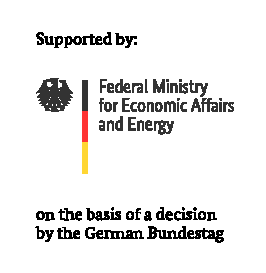
\includegraphics[width=7.9cm]{bmwe-supported-by-en.pdf}\par
          \vfill
          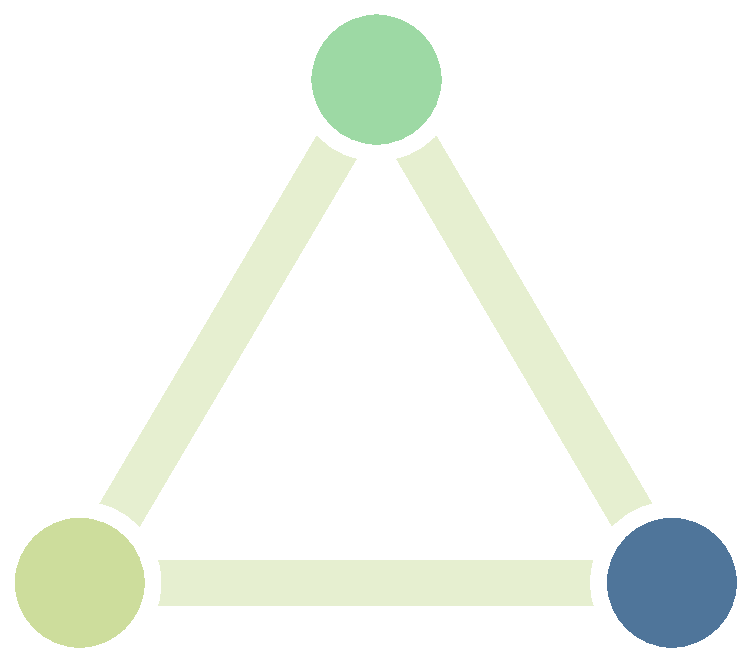
\includegraphics[width=6.4cm]{resilient-triangle.pdf}
      \end{minipage}\hspace{1.5em}%
      \usebox{\qrcolumn}}%
\end{minipage}
\par
\vspace{0.4cm}


%----------------------------------------------------------------------------------------
%	POSTER BODY
%----------------------------------------------------------------------------------------

% three equal-height columns: each column is set into a box first, then all
% are output with the height of the tallest one; the \vfill between boxes
% spreads the remaining space evenly, so all bottom borders line up
\newsavebox\posterColA \newsavebox\posterColB \newsavebox\posterColC
\newlength\posterColW \setlength\posterColW{\dimexpr(\linewidth-2\columnsep)/3\relax}
\newlength\posterColH
\setbox\posterColA=\vbox{\hsize=\posterColW \linewidth=\hsize
%----------------------------------------------------------------------------------------
%	COLUMN 1: MOTIVATION, SCENARIOS, METHOD, COSTS
%----------------------------------------------------------------------------------------

\begin{posterbox}{Motivation}

\noindent North Rhine-Westphalia (NRW) hosts much of Germany's steel, cement, lime, chemical and waste incineration capacity. Part of their process emissions is unavoidable, so carbon capture, transport, storage and use (CCS/CCU) are needed for climate neutrality by 2045. Without domestic storage, captured \ce{CO2} can be piped to the North Sea, and NRW lies on the route from southern Germany. In this RESILIENT case study (TU Berlin, Fraunhofer ISI, IN4climate.NRW), we ask:
\begin{itemize}
  \item How should a \textbf{\ce{CO2} pipeline network} in NRW and \\Germany be built up, and how is it used?
  \item How do the planned \textbf{PCI-PMI} \ce{CO2} pipeline projects \\compare with an \textbf{endogenously optimised} network?
  \item How much \ce{CO2} \textbf{passes through} NRW from other\\regions?
\end{itemize}

\end{posterbox}
\vfill
\begin{posterbox}{Scenarios}

\noindent Industrial demand and emissions come from the bottom-up model FORECAST \cite{fleiterMethodologyBottomupModelling2018}, soft-linked into PyPSA-Eur. \textbf{HtA+} keeps more fossil routes in place (steam crackers, \ce{CH4}-based direct reduction, blast furnaces) and extends the adoption of carbon capture.

% scenario schematic: one column per scenario, bars span the scenarios that
% share a setting; light red marks what changes compared with the 1.a baseline
% (not a numbered figure, no caption)
\par\smallskip\noindent
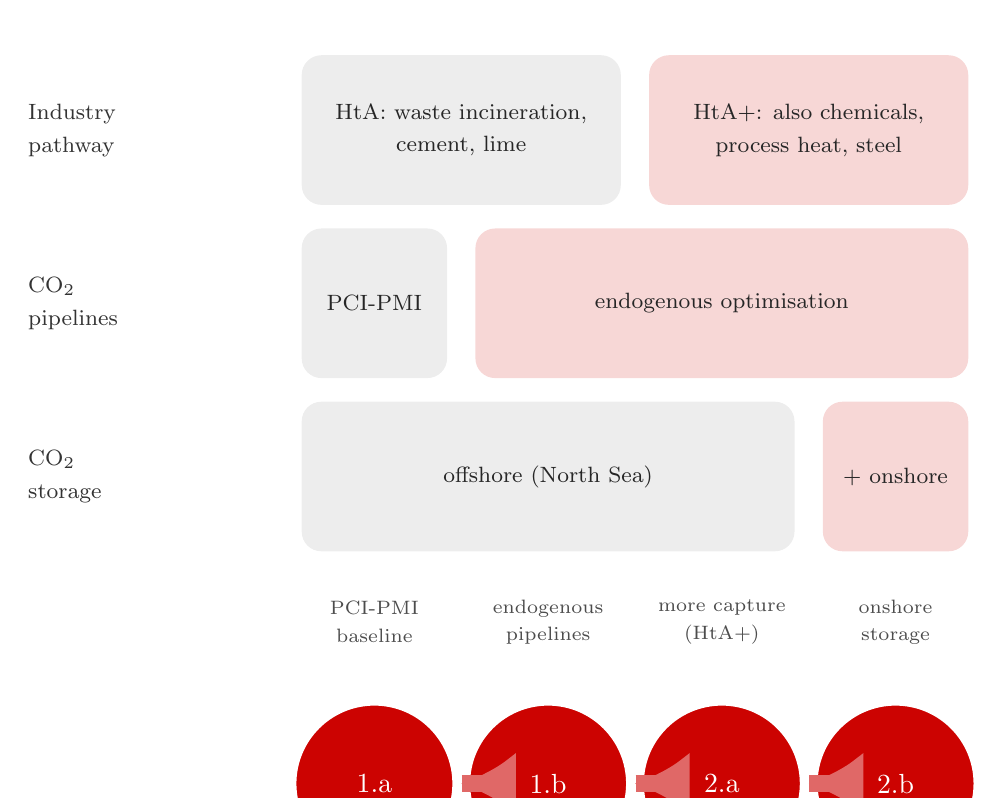
\begin{tikzpicture}[
    font=\footnotesize,
    bar/.style={rounded corners=2.5mm,minimum height=1.9cm,inner sep=0.2em,
      align=center,text=black!85},
    base/.style={bar,fill=black!7},
    change/.style={bar,fill=red100!16},
    scen/.style={circle,fill=red100,text=white,font=\normalsize\bfseries,
      minimum size=2.1cm,inner sep=0pt},
    rowlab/.style={anchor=west,align=left,inner xsep=0pt,font=\footnotesize\bfseries,text=black!80},
  ]
  \pgfmathsetlengthmacro{\lab}{3.3cm}          % width of the row labels
  \pgfmathsetlengthmacro{\col}{(\linewidth-\lab)/4} % width of one scenario column
  \pgfmathsetlengthmacro{\gap}{0.18cm}
  \pgfmathsetlengthmacro{\rowh}{2.2cm}
  % x centre of scenario column k (0..3)
  \newcommand{\cx}[1]{\lab+(#1+0.5)*\col}
  % bar from column a to column b (inclusive) in row r
  \newcommand{\spanbar}[5]{%
    \node[#4,minimum width={(#2-#1+1)*\col-2*\gap}]
      at ({\lab+(#1+#2+1)/2*\col},{-#3*\rowh}) {#5};}

  % rows
  \node[rowlab] at (0,{-1*\rowh}) {Industry\\pathway};
  \node[rowlab] at (0,{-2*\rowh}) {\ce{CO2}\\pipelines};
  \node[rowlab] at (0,{-3*\rowh}) {\ce{CO2}\\storage};

  \spanbar{0}{1}{1}{base}{\textbf{HtA}: waste incineration,\\cement, lime}
  \spanbar{2}{3}{1}{change}{\textbf{HtA+}: also chemicals,\\process heat, steel}
  \spanbar{0}{0}{2}{base}{PCI-PMI}
  \spanbar{1}{3}{2}{change}{endogenous optimisation}
  \spanbar{0}{2}{3}{base}{offshore (North Sea)}
  \spanbar{3}{3}{3}{change}{+ onshore}

  % what each scenario changes (inside the box) ...
  \foreach \k/\what in {0/PCI-PMI\\baseline, 1/endogenous\\pipelines,
                        2/more capture\\(HtA+), 3/onshore\\storage}{
    \node[font=\scriptsize,align=center,text=black!70] at ({\cx{\k}},{-3.5*\rowh-0.75cm}) {\what};
  }
  % ... and the scenario circles, centred on the bottom edge of the box so
  % they float half on the box, half on the page background
  \pgfmathsetlengthmacro{\cy}{-3.5*\rowh-1.75cm-1.05cm}
  \foreach \k/\name in {0/1.a,1/1.b,2/2.a,3/2.b}{
    \node[scen,draw=white,line width=1.2mm,overlay] (s\k) at ({\cx{\k}},\cy) {\name};
  }
  \foreach \a/\b in {0/1,1/2,2/3}{
    \draw[-{Latex[length=7mm,width=8mm]},line width=2.2mm,red100!60,overlay] (s\a) -- (s\b);
  }
  % circles and arrows are overlays (not part of the size); the picture ends
  % at the circle centres plus the box's bottom padding, so the box edge runs
  % through the circle centres and the lower halves hang out of the box
  \path (0,{-1*\rowh+1.3cm}) (0,{\cy+0.5em});
\end{tikzpicture}
\end{posterbox}
\vspace{0.4cm} % room for the lower half of the scenario circles
% Delaunay map on a white card floating out of the bottom-right corner
\vfill
\begin{posterbox}[overlay={%
    \node[anchor=south east,inner sep=0pt]
      at ([xshift=1.2cm,yshift=-1.9cm]frame.south east) {%
      \tcbox[enhanced,colback=white,colframe=red100,boxrule=0.8mm,arc=4mm,
        left=0.3em,right=0.3em,top=0.3em,bottom=0.3em,nobeforeafter]{%
        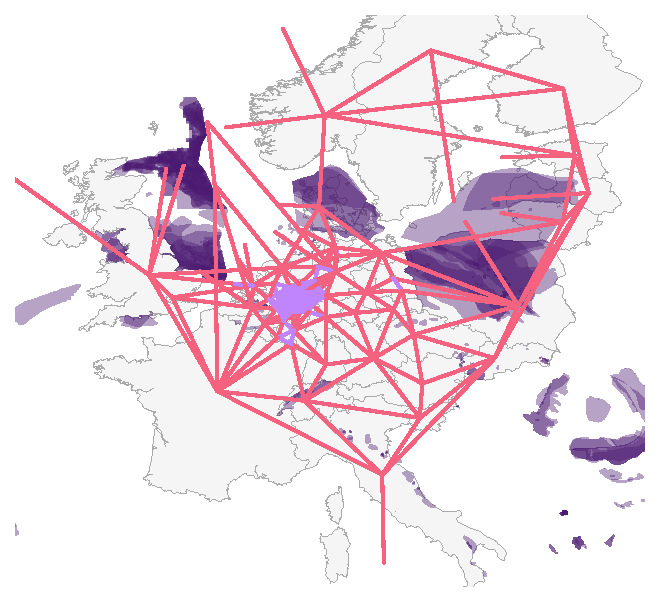
\includegraphics[width=11.8cm]{co2_delaunay_2035.pdf}}};}]{Model setup}

\noindent We use the open-source, sector-coupled model PyPSA-Eur \cite{horschPyPSAEurOpenOptimisation2018,neumannPotentialRoleHydrogen2023,hofmannH2CO2Network2025}, covering all energy sectors in around 80 regions: NRW by county (NUTS3), the rest of Germany by state, and 19 neighbouring countries.

\begin{itemize}
  \item Myopic 2035--2040--2045, 1460 time steps per year; planned power grid, \ce{H2} pipelines optimised.
\end{itemize}
\noindent
\begin{minipage}[t]{0.5\linewidth}
\raggedright
\begin{itemize}
  \item Offshore storage at 30\,\euro/t, 100--250\,Mt/a.
  \item Pipeline candidates on a Delaunay graph (right), rounded to DN400 ($\approx$\,9\,Mt/a) or DN700 ($\approx$\,28\,Mt/a).
\end{itemize}
\end{minipage}
\end{posterbox}}

\setbox\posterColB=\vbox{\hsize=\posterColW \linewidth=\hsize
%----------------------------------------------------------------------------------------
%	COLUMN 2: NETWORK, PIPELINES, CAPTURE
%----------------------------------------------------------------------------------------

\begin{posterbox}{\ce{CO2} network}

\noindent In 2045, NRW's steel, refinery and cement sites are connected to a network that leads mainly west towards the Netherlands and north towards Bremen, and from there to offshore storage in the North Sea (Fig.~\ref{fig:maps}). Some routes appear in all scenarios, e.g.\ the westward corridor to the Netherlands and Belgium and the transit corridors in south-eastern NRW. Some captured \ce{CO2} stays in NRW as feedstock for methanol and Fischer-Tropsch fuels.

\begin{center}
    % widths proportional to the map aspect ratios -> equal heights, top aligned
    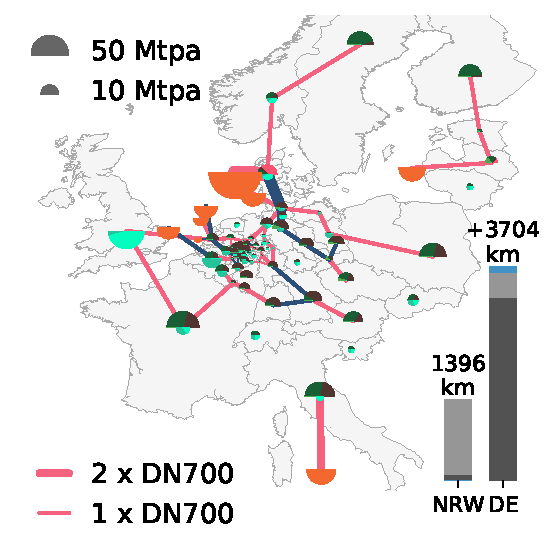
\includegraphics[width=0.4976\linewidth,valign=t]{co2_network_2a_2045_poster.pdf}\hfill
    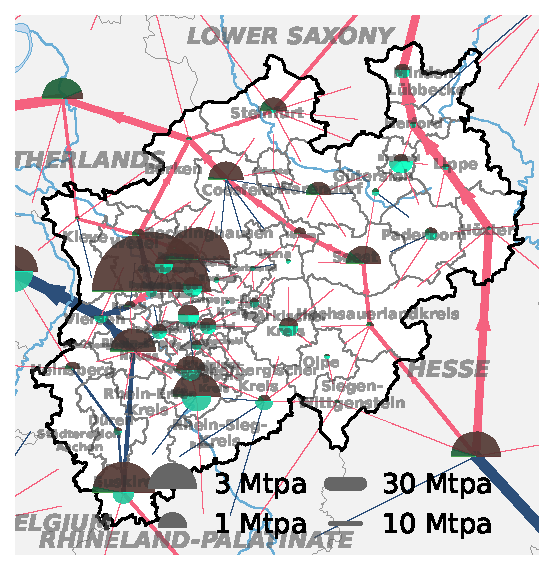
\includegraphics[width=0.4824\linewidth,valign=t]{co2_flow_nrw_2a_2045_poster.pdf}\\[0.6em]
    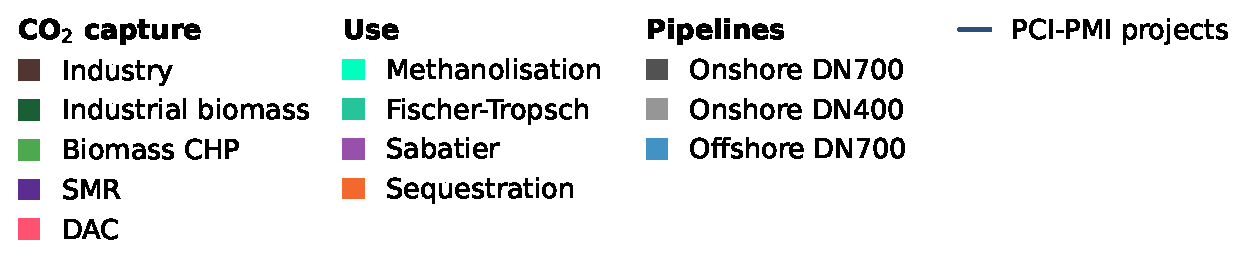
\includegraphics[width=0.95\linewidth]{co2_network_legend_2a_2045_poster.pdf}
    \captionof{figure}{Scenario 2.a (HtA+, endogenous pipelines), 2045: \ce{CO2} capture (upper half-circles) and use or storage (lower half-circles), pipeline capacities in Europe (left) and annual net \ce{CO2} flows in NRW (right, arrows: flow direction). Blue: PCI-PMI projects.}
    \label{fig:maps}
\end{center}

\end{posterbox}
\vfill
\begin{posterbox}{Pipeline sizing}

\noindent The fixed PCI-PMI network (1.a) has about 4\,400--4\,600\,km of pipelines in Germany, but its onshore DN400 pipes run below 15\,\% of capacity in every year. With endogenous expansion (1.b), the network is 2\,300--2\,700\,km long and better utilised. DN700-equivalent pipes are enough for transport between regions, and offshore collector lines run at constantly high utilisation (Fig.~\ref{fig:pipelines}).

\begin{center}
    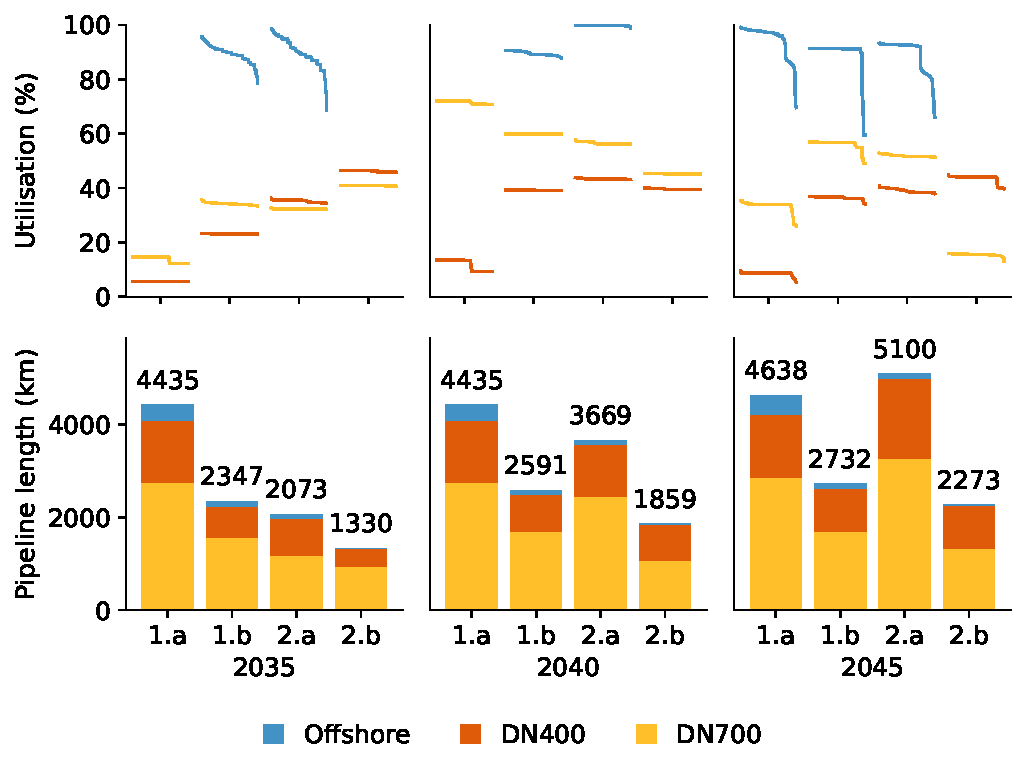
\includegraphics[width=\linewidth,trim={7.2bp 0 6.8bp 0},clip]{co2_pipeline_utilisation_dashboard_de_poster.pdf}
    \captionof{figure}{Germany (incl.\ NRW): annual utilisation duration curves per pipeline (top) and pipeline lengths by type (bottom).}
    \label{fig:pipelines}
\end{center}

\end{posterbox}}

\setbox\posterColC=\vbox{\hsize=\posterColW \linewidth=\hsize
%----------------------------------------------------------------------------------------
%	COLUMN 3: TRANSIT, COSTS, TAKE-AWAYS, PROJECT
%----------------------------------------------------------------------------------------

\begin{posterbox}{\ce{CO2} transit through NRW}

\noindent Much of the \ce{CO2} crossing NRW's borders is \textbf{transit} from Hesse, Rhineland-Palatinate and southern Germany. We derive transit from the hourly pipeline flows with proportional-sharing flow tracing \cite{bialekTracingFlowElectricity1996,horschFlowTracingTool2018}; the whiskers in Fig.~\ref{fig:transit} show the possible range.
\begin{itemize}
  \item In 2045, 23--46\,Mt/a of \ce{CO2} pass through NRW in the offshore-only scenarios (1.a--2.a). Almost all imported \ce{CO2} leaves NRW again.
  \item In HtA+ (2.a), NRW's own exports grow to about 41\,Mt/a on top of transit.
  \item With onshore storage (2.b), transit almost disappears (below 5\,Mt/a).
\end{itemize}

\begin{center}
    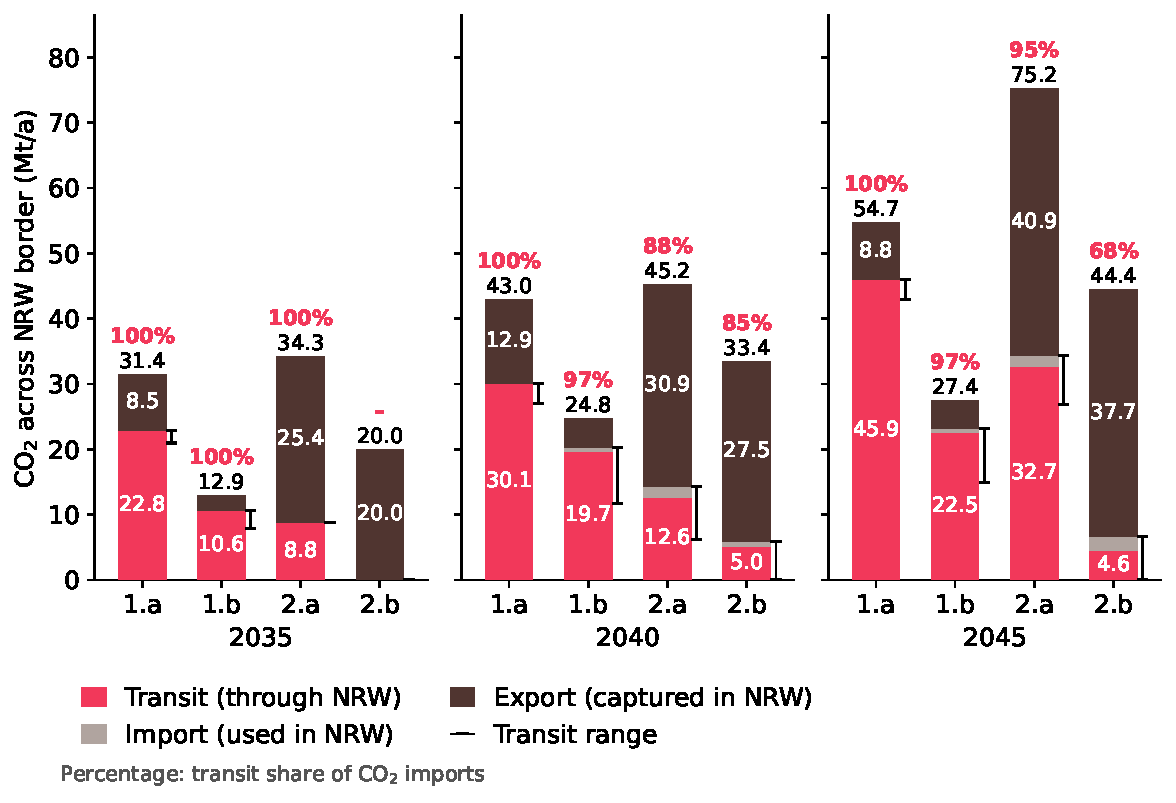
\includegraphics[width=\linewidth]{co2_transit_nrw_dashboard_poster.pdf}
    \captionof{figure}{\ce{CO2} flows across the NRW border: transit (red), imports used in NRW (grey) and exports of \ce{CO2} captured in NRW (brown). Percentages: transit share of \ce{CO2} imports into NRW.}
    \label{fig:transit}
\end{center}

\end{posterbox}
\vfill
\begin{posterbox}{System costs}

\noindent An optimised pipeline network lowers annual European system costs by 19--26\,bn\,\euro{} compared with the fixed PCI-PMI network (1.b vs.\ 1.a), mainly through lower \ce{CO2} infrastructure costs and less DAC. Onshore storage (2.b) saves a further $\sim$8\,bn\,\euro/a compared with 2.a in 2045 and more than halves the pipeline investment (Fig.~\ref{fig:costs}).

\begin{center}
    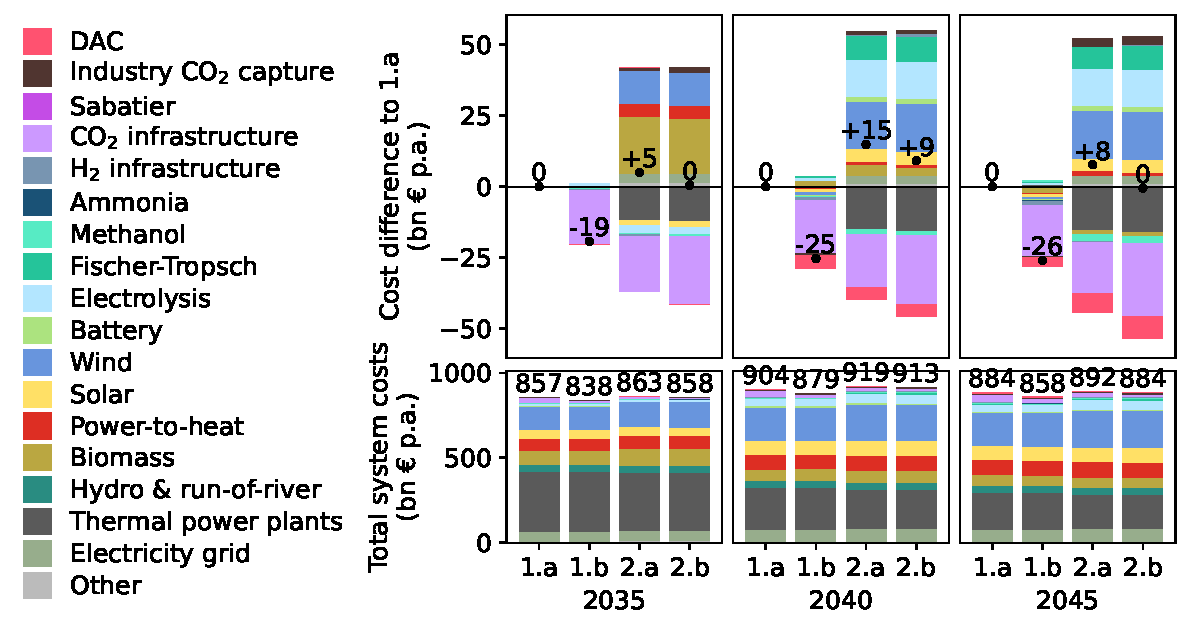
\includegraphics[width=\linewidth,trim={11.5bp 0 6.8bp 0},clip]{costs_overview_stacked_poster.pdf}
    \captionof{figure}{Cost difference to scenario 1.a (top) and total annualised system costs (bottom) in bn\,\euro/a.}
    \label{fig:costs}
\end{center}

%---------------------------------------------------------------------------------------
\end{posterbox}}

\setlength\posterColH{\dimexpr\ht\posterColA+\dp\posterColA}
\ifdim\dimexpr\ht\posterColB+\dp\posterColB>\posterColH \setlength\posterColH{\dimexpr\ht\posterColB+\dp\posterColB}\fi
\ifdim\dimexpr\ht\posterColC+\dp\posterColC>\posterColH \setlength\posterColH{\dimexpr\ht\posterColC+\dp\posterColC}\fi
\vspace*{0.5cm}
\noindent
\vtop{\kern0pt\vbox to \posterColH{\unvbox\posterColA}}\hspace{\columnsep}%
\vtop{\kern0pt\vbox to \posterColH{\unvbox\posterColB}}\hspace{\columnsep}%
\vtop{\kern0pt\vbox to \posterColH{\unvbox\posterColC}}\par


%----------------------------------------------------------------------------------------
%	TAKE-AWAYS (full width)
%----------------------------------------------------------------------------------------
\vspace{1.8em}
\begin{tcolorbox}[postertab,title={Take-aways},colback=takegrey,colframe=takedark,arc=4mm,boxrule=1mm,toprule=1.2mm,left=1.1em,right=1.1em,top=1em,bottom=0.8em,before skip=0pt,after skip=0.6em,boxed title style={colback=takedark,colframe=takedark}]
\begin{multicols}{3}
\raggedcolumns
\begin{enumerate}
  \item \textbf{Robust corridors}: the westward link to the Netherlands and Belgium and the transit corridors in south-eastern NRW appear in all scenarios.
  \item \textbf{NRW: start small}, with 1--2 DN400 feeder pipes ($\approx$\,9\,Mt/a each), connecting the largest emitters first: steel, then refineries and cement.
  \item \textbf{NRW is a transit hub}: up to 46\,Mt/a of \ce{CO2} from other regions crosses NRW unless onshore storage is available.
  \vfill\columnbreak
  \item \textbf{PCI-PMI \ce{CO2} projects are oversized}, mainly in capacity and slightly in length. DN700-equivalent pipes ($\approx$\,28\,Mt/a) are enough between regions; offshore collection points need larger or parallel pipes.
  \vspace{1.2em}
  \item \textbf{Onshore storage} in Germany and neighbouring countries more than halves pipeline investment and saves $\sim$8\,bn\,\euro/a.
  \vfill\columnbreak
  \item \textbf{Capture and DAC}: well-sized capture units can run above 70\,\% utilisation (15--50\,Mt/a in NRW, 60--130\,Mt/a in Germany). DAC is built mainly in neighbouring countries, and an optimised network beyond PCI-PMI greatly reduces Europe's DAC needs.
  \item \textbf{CCU and DAC alone are not enough}: transport, storage and local use are all needed, including to supply aviation and shipping fuels.
\end{enumerate}
\end{multicols}
\end{tcolorbox}

%----------------------------------------------------------------------------------------
%	ACKNOWLEDGEMENTS & REFERENCES
%----------------------------------------------------------------------------------------
% acknowledgement (left third) and references (right two thirds, 2 columns),
% all top-aligned
% (\singlespacing must come before the size command: it re-selects \@currsize)
\noindent
\begin{minipage}[t]{0.31\linewidth}
  \vspace{0pt}
  {\singlespacing\scriptsize This work was supported by the German Federal Ministry for Economic Affairs and Energy (BMWE) under Grant No.\ 03EI4083A (RESILIENT). This project has been funded by partners of the CETPartnership (https://cetpartnership.eu) through the Joint Call 2022. As such, this project has received funding from the European Union's Horizon Europe research and innovation programme under grant agreement no.\ 101069750.\par}
\end{minipage}\hfill
\begin{minipage}[t]{0.66\linewidth}
  \vspace{0pt}
  \singlespacing\scriptsize
  \setlength{\columnsep}{2em}
  \setlength{\multicolsep}{0pt}
  \begin{multicols}{2}
    % drop the default "References" section heading of thebibliography
    \renewcommand{\section}[2]{}%
    \setlength{\itemsep}{0pt}%
    % no extra space above the list, so references line up with the acknowledgement
    \makeatletter\def\@openbib@code{\setlength{\topsep}{0pt}\setlength{\partopsep}{0pt}\setlength{\itemsep}{0.15em}}\makeatother
    \bibliographystyle{plain}
    \bibliography{references}
  \end{multicols}
\end{minipage}

% footer bar in the same style as the boxes (rounded, padded), pinned to the
% bottom of the page outside the text flow so it does not compete for space
\begin{tikzpicture}[remember picture,overlay]
  \node[anchor=south west,inner sep=0pt]
    % (+1in compensates the -1in \hoffset/\voffset set by a0poster.cls, which
    %  TikZ's "current page" node does not account for)
    at ([xshift=\leftbleed+1in,yshift=1.87cm+1in]current page.south west) {%
    \begin{tcolorbox}[enhanced,colback=red100,colframe=red100,boxrule=0pt,arc=4mm,
      width=\textwidth,left=1.5em,right=1.5em,top=0.5em,bottom=0.5em,halign=center,
      before skip=0pt,after skip=0pt]
      \color{white}
      \textbf{Contact:} Bobby Xiong (xiong@tu-berlin.de) \quad
      \textbf{Keywords:} open-source $\cdot$ energy system modelling $\cdot$ carbon capture $\cdot$ \ce{CO2} pipelines $\cdot$ industry $\cdot$ North Rhine-Westphalia $\cdot$ PCI-PMI
    \end{tcolorbox}};
\end{tikzpicture}

\end{document}
